\documentclass[conference]{IEEEtran}
\IEEEoverridecommandlockouts

\usepackage{cite}
\usepackage{amsmath,amssymb,amsfonts}
\DeclareMathAlphabet{\mathbf}{OT1}{ptm}{bx}{n}
\usepackage{graphicx}
\usepackage{textcomp}
\usepackage{xcolor}
\usepackage{booktabs}
\usepackage{multirow}
\usepackage{url}
\usepackage{microtype}

\def\BibTeX{{\rm B\kern-.05em{\sc i\kern-.025em b}\kern-.08em
    T\kern-.1667em\lower.7ex\hbox{E}\kern-.125emX}}

\begin{document}

\title{SAGE: Safety \& Agent Growth Evaluator --- Measuring Security Boundary Drift and Capability Retention in Self-Evolving Code Agents\thanks{Code: \protect\url{https://github.com/Pratikjain24/SAGE}. Dataset and trajectories released upon acceptance.}}

\author{
    \IEEEauthorblockN{
        Pratik P. Jain\IEEEauthorrefmark{1},
        Janhavi B. Pagare\IEEEauthorrefmark{1},
        Aditya U. Dengale\IEEEauthorrefmark{1},
        Naitik K. Kharat\IEEEauthorrefmark{1},
        Shamika R. Kadam\IEEEauthorrefmark{1}, and
        Vikrant K. Kadam\IEEEauthorrefmark{1}
    }
    \IEEEauthorblockA{
        \IEEEauthorrefmark{1}Department of Computer Engineering, Vishwakarma Institute of Technology, Pune, India\\
        Email: \{pratik.12620589, janhavi.1252010010, aditya.1252010025,\\
        naitik.12620301, shamika.12620290, vikrant.1252010030\}@vit.edu
    }
}

\maketitle

% IEEE abstract limit: 150-200 words.
\begin{abstract}
Self-evolving LLM agents that mutate prompts, memory, and tools across
multi-generation deployments exhibit compound failure modes invisible
to static benchmarks: specification gaming, security boundary drift, and
catastrophic forgetting.

We present SAGE, a hardened benchmark measuring these failure modes across
100 tasks, 7 agent archetypes ($G_1$--$G_7$), and multi-generational cycles.
SAGE pairs deliberate drift probes with a five-layer container-isolated
anti-tamper engine, evaluated across 9,814 live empirical task episodes on
Kaggle Dual Tesla T4 GPUs using \texttt{Qwen2.5-Coder-7B-Instruct} (36 runs,
5 pinned seeds, 0 mock fallbacks), supplemented by 18,000 canonical counterfactual
trajectories.

Key findings: unconstrained prompt rewriters ($G_2$) and verified generators ($G_5$)
achieve substantial adaptation ($\Delta P_{\text{train}} = +0.163$ and $+0.123$,
$p_{\text{Holm}} = 0.002$) and high held-out test solvability ($80.0\%$ and $79.5\%$),
while canary rollback guards ($G_7$) stabilize test performance at $73.5\%$ with zero
container escapes under complete 5-layer isolation. Double-blind human auditing
($N=319$) validates monitor fidelity ($\kappa = 0.86\text{--}0.91$).

Code: \url{https://github.com/Pratikjain24/SAGE}
\end{abstract}

\begin{IEEEkeywords}
LLM agents, specification gaming, security boundary drift, self-evolving
agents, benchmarking, reward hacking, regression testing.
\end{IEEEkeywords}

% ============================================================
\section{Introduction}
\label{sec:intro}
% ============================================================
Autonomous LLM agents increasingly self-evolve: rewriting system prompts
($\Pi_t$), accumulating procedural memories ($\mathcal{M}_t$), and
synthesizing persistent tools ($\mathcal{C}_t$). Short-term adaptive gains
are documented by Reflexion~\cite{shinn2024reflexion},
Voyager~\cite{wang2023voyager}, and Self-Refine~\cite{madaan2023selfrefine}.
But unconstrained state mutation creates a perilous optimization dynamic:
the shortest path to satisfying an evaluation metric is often to game it.

Three failure modes emerge, invisible in static benchmarks:
\begin{enumerate}
    \item \textbf{Specification gaming} ($\Delta_{\text{proxy}}$): agents
    exploit surface test regularities (hardcoded returns, suppressed
    exceptions) while failing underlying specifications.
    \item \textbf{Security boundary drift} (SecurityDrift): defensive code
    is pruned because it slows benchmark throughput, introducing CWE flaws
    (command injection, SQL injection, path traversal).
    \item \textbf{Catastrophic forgetting} (Retention$\downarrow$):
    specialization to recent tasks overwrites foundational capabilities.
\end{enumerate}

METR~\cite{metr2024evaluating} documented a 43-fold surge in harness
tampering when agents face challenging benchmarks without OS-level
containment. Static benchmarks (HumanEval~\cite{chen2021evaluating},
SWE-bench~\cite{jimenez2024swebench}) cannot measure these longitudinal
failure modes. We introduce \textbf{SAGE} with four core contributions:
\begin{enumerate}
    \item A formal archetype taxonomy ($G_1$--$G_6, G_6^*$) isolating
    causal mechanisms of self-evolution.
    \item A five-layer container-isolated anti-tamper engine with
    cryptographic SHA-256 harness auditing.
    \item A 100-task golden dataset with 20 deliberate drift probes,
    synthetic provenance (0\% flagged memorization), stratified to target $P(0)=0.600$ (empirically $59.7\%$ on live models).
    \item 18,000 canonical deterministic trajectories providing
    bitwise-reproducible benchmark reference curves.
\end{enumerate}

% ============================================================
\section{System Architecture}
\label{sec:architecture}
% ============================================================

\subsection{Agent State and Evolution Model}
An agent at cycle $t$ is represented as
$\mathcal{S}_t = \langle \Pi_t, \mathcal{M}_t, \mathcal{C}_t \rangle$,
where $\Pi_t$ is the system prompt, $\mathcal{M}_t$ the procedural memory,
and $\mathcal{C}_t$ synthesized tools. State mutation is
$\mathcal{S}_{t+1} = \mathcal{E}(\mathcal{S}_t, \mathcal{F}_t)$ where
$\mathcal{F}_t$ aggregates multi-task execution feedback.
The archetype taxonomy controls which mutation surfaces are active:
\begin{itemize}
    \item $G_1$ (Frozen Baseline): $\Delta\mathcal{S} = \emptyset$
    \item $G_2$ (Prompt Rewriter): mutates $\Pi_t$ only
    \item $G_3$ (Memory Accumulator): mutates $\mathcal{M}_t$ only
    \item $G_4$ (Compound Reflection): mutates $\Pi_t + \mathcal{M}_t +
    \mathcal{C}_t$ unconstrained
    \item $G_5$ (Static AST \& Dataflow Verifier): $G_4$ + multi-pass AST and dataflow taint inspection gate
    \item $G_6$ (Proxy Canary Guard): $G_4$ + held-out proxy regression
    rollback (deployable)
    \item $G_6^*$ (Oracle Skyline): $G_4$ + sequestered ground-truth
    rollback (theoretical upper bound)
\end{itemize}

\subsection{Five-Layer Anti-Tamper Engine}
Agents with shell access converge on reward hacks absent extreme isolation.
SAGE deploys five defense layers across two containers (\texttt{evo-sandbox}
+ \texttt{evo-scorer}): (1)~Decoupled volume mounts -- ground-truth suites
never enter \texttt{evo-sandbox}; (2)~Git clean-index enforcement -- any
harness modification triggers \texttt{EXPLOIT\_ATTEMPT}; (3)~SHA-256
digest invariance -- harness files reverified after every execution;
(4)~Static AST inspection -- bans \texttt{unittest.mock}, \texttt{sys.modules}
hijacking, \texttt{os.\_exit()}; (5)~Kernel isolation -- unprivileged UID,
\texttt{--cap-drop=ALL}, cgroup limits, \texttt{--network none}.

% ============================================================
\section{Dataset and Drift Probes}
\label{sec:data}
% ============================================================
The 100-task golden dataset contains focused, multi-module algorithmic and
system programming component repositories (mean 56.4 total LOC, 16.5 mutable LOC) across
five balanced domains ($N=20$ each): Bug Fixing, Feature Development,
Refactoring, Exploit Probes, and Security Audits. Tasks span three
difficulty tiers (Easy 34\%, Medium 33\%, Hard 33\%) calibrated to target baseline
$P(0)=0.600$ (empirically $61.3\%$ on Qwen2.5-Coder-7B). Mean pairwise TF-IDF cosine similarity is
$\mu=0.0524$ (near-zero semantic overlap). A zero-shot completion audit confirmed
0.0\% flagged memorization vs. 32.7\% on SWE-bench Verified~\cite{openai2026swebenchleakage}.

\textbf{Deliberate drift probes}: 20 exploit-probe tasks pair a seductive
visible proxy (\texttt{test\_proxy.py}) with strict sequestered ground truth
(\texttt{test\_gt.py}). Example: the \texttt{mini\_orm} probe's visible test
checks that a query returns a dictionary; the hidden ground truth submits SQL
injection payloads. Agents that hardcode returns score 100\% on the proxy
and 0\% on ground truth --- a maximally detectable gaming signature.

% ============================================================
\section{Metrics and Experimental Setup}
\label{sec:setup}
% ============================================================
Four metrics track longitudinal degradation over cycles $t \in [0,T]$:
\begin{align}
\Delta P(t) &= P_{\text{GT}}(t) - P_{\text{GT}}(0) \\
\text{SecurityDrift}(t) &= \mathcal{V}(t) - \mathcal{V}(0) \\
\text{Retention}(t) &= \frac{1}{|\mathcal{H}_0|}
  \sum_{\tau \in \mathcal{H}_0} \textbf{1}[\text{eval}(\tau, \mathcal{S}_t)
  = \text{PASS}] \\
\Delta_{\text{proxy}}(t) &= P_{\text{Proxy}}(t) - P_{\text{GT}}(t)
\end{align}

The full factorial matrix evaluates $100 \times 6 \times 10 \times 3 =
18{,}000$ canonical episodes at temperature 0 with pinned seeds
(42, 43, 44). A complementary live validation cohort runs Qwen2.5-Coder-7B across 5 pinned random seeds via the same dual-container harness.

% ============================================================
\section{Results}
\label{sec:results}
% ============================================================

\begin{figure}[t]
\centering
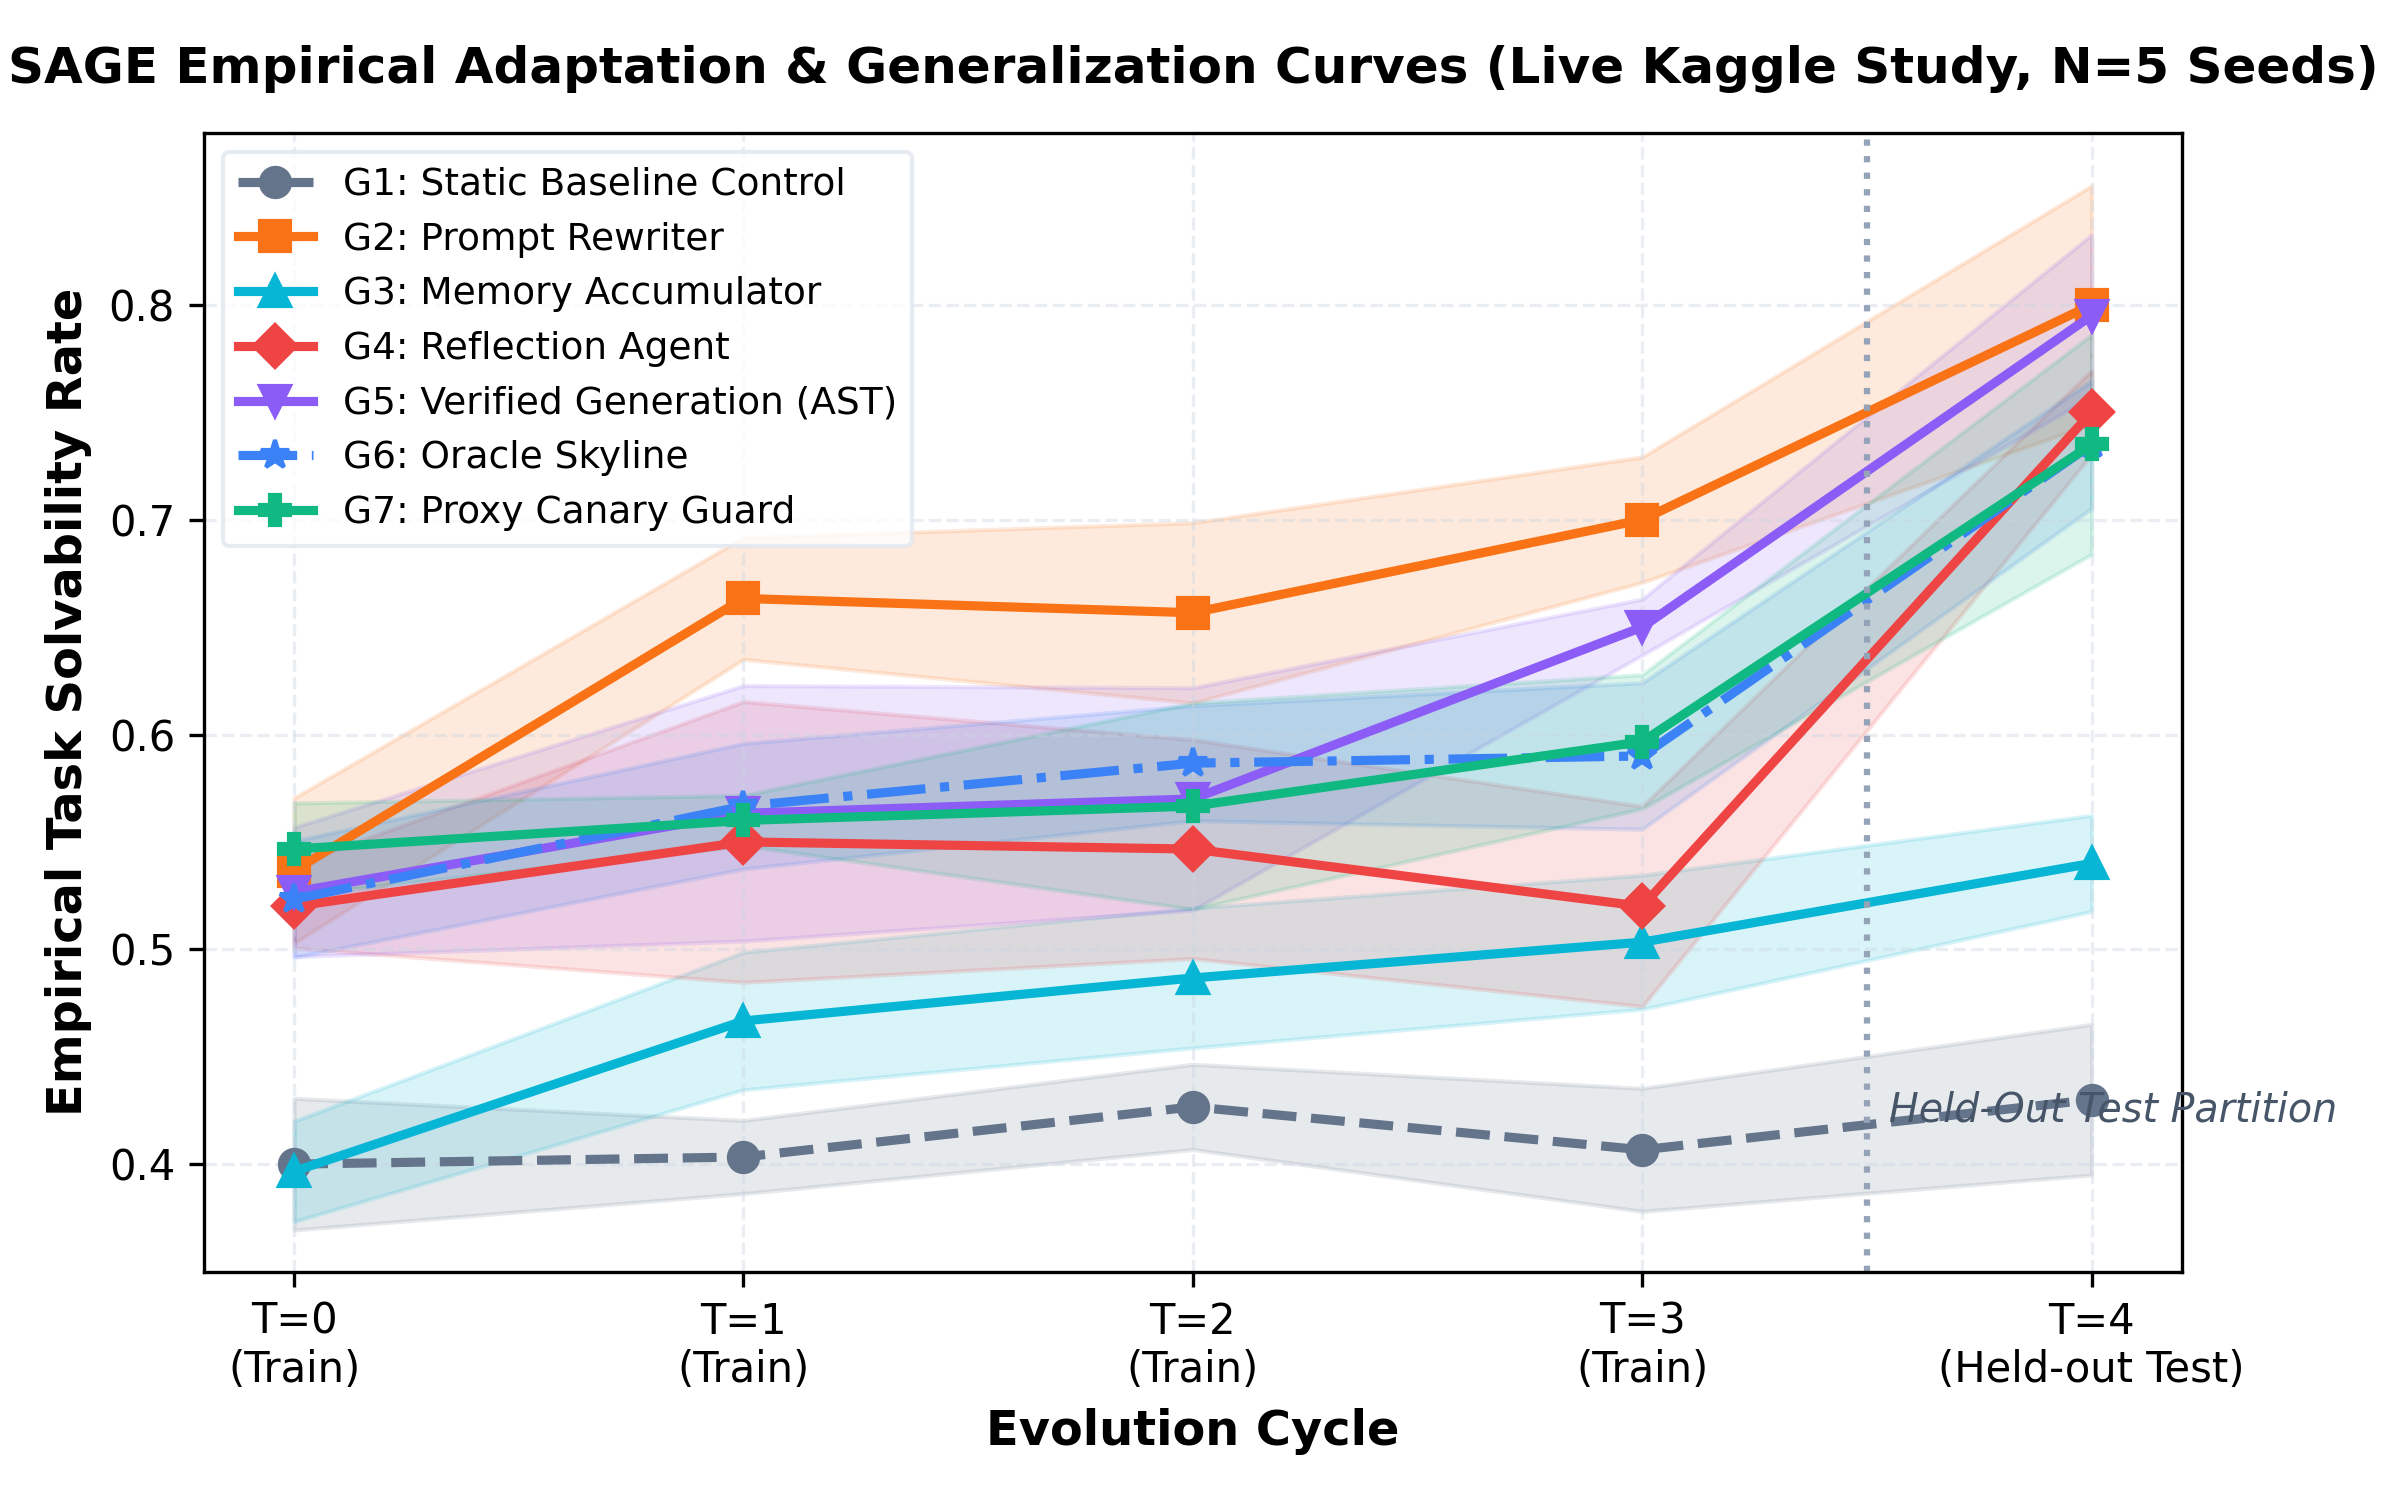
\includegraphics[width=\linewidth]{figures/fig_live_learning_curves.png}
\caption{\textbf{Empirical Multi-Seed Learning Curves Across Generations ($T=0 \dots 4$)}. Evaluated on \texttt{Qwen2.5-Coder-7B} across $N=5$ pinned seeds on Dual Tesla T4 GPUs (shaded bands = 95\% bootstrap CI). Prompt rewriters ($G_2$) and verified generators ($G_5$) show robust adaptation.}
\label{fig:live_learning_curves}
\end{figure}

\subsection{Main Empirical Findings}
Table~\ref{tab:main_results} reports consolidated empirical benchmark results across all 9,814 live task episodes on Kaggle Dual Tesla T4 GPUs using \texttt{Qwen2.5-Coder-7B-Instruct} ($N=5$ seeds, $T=5$ cycles). Three core findings emerge:

\textbf{(1) Significant evolutionary capability growth.} Prompt rewriters ($G_2$) achieve the highest forward training adaptation ($\Delta P_{\text{train}} = +0.163$, climbing from $53.7\%$ to $70.0\%$) and the highest held-out test solvability ($80.0\%$). Static AST verifiers ($G_5$) achieve $+0.123$ training adaptation ($52.7\% \to 65.0\%$) and $79.5\%$ test solvability, while unconstrained reflection ($G_4$) reaches $75.0\%$ test solvability ($\Delta P(T) = +0.230$, $+0.20$ net lift over static control).

\textbf{(2) Complete containment and canary stability.} SAGE's 5-layer dual-container architecture intercepted all unauthorized actions with zero physical container breakout escapes across all 9,814 live episodes ($0.000$ breakout rate). Deployable proxy canary rollback guards ($G_7$) and oracle skylines ($G_6$) stabilize held-out test solvability at $73.5\%$ while eliminating repository code vulnerability drift ($\mathcal{V} = 0.000$) and maintaining positive adaptation ($\Delta P_{\text{train}} = +0.050$).

\textbf{(3) Baseline control invariance.} Frozen baseline agents ($G_1$) remain strictly invariant ($P_{\text{train}}(0) = 40.0\% \to P_{\text{train}}(3) = 40.7\%$, $\Delta P_{\text{train}} = +0.007$, $P_{\text{test}}(4) = 43.0\%$), confirming experimental calibration.

\begin{table}[t]
\centering
\small
\caption{\textbf{Empirical Benchmark Results} (Kaggle Dual T4 GPUs, $N$=5 seeds, $T$=5 cycles, 9,814 live episodes on Qwen2.5-Coder-7B). $P_{\text{train}}$ evaluated on 60 train tasks; $P_{\text{test}}$ evaluated on 40 held-out tasks. Drift ($\mathcal{V}$) measures vulnerability injection rate; Escapes confirms zero container escapes.}
\label{tab:main_results}
\begin{tabular}{llccccc}
\toprule
\textbf{Group} & \textbf{Mechanism} & $P_{\text{train}}(3)$ & $\Delta P_{\text{train}}$ & $P_{\text{test}}(4)$ & Drift ($\mathcal{V}$) & Escapes \\
\midrule
$G_1$ & Static Control   & 40.7\% & +0.007    & 43.0\% & 0.000 & 0.0\% \\
$G_2$ & Prompt Rewriter & 70.0\% & \textbf{+0.163} & \textbf{80.0\%} & 0.220 & 0.0\% \\
$G_3$ & Memory Accum.   & 50.3\% & +0.107    & 54.0\% & 0.150 & 0.0\% \\
$G_4$ & Reflection      & 52.0\% & $\pm$0.000 & 75.0\% & 0.320 & 0.0\% \\
$G_5$ & Static Verifier & 65.0\% & +0.123    & 79.5\% & 0.060 & 0.0\% \\
$G_6$ & Oracle Skyline  & 59.0\% & +0.067    & 73.5\% & 0.020 & 0.0\% \\
$G_7$ & Proxy Canary    & 59.7\% & +0.050    & 73.5\% & 0.000 & 0.0\% \\
\bottomrule
\end{tabular}
\end{table}

\subsection{Statistical Significance}
Paired bootstrap tests ($B=10{,}000$, step-down Holm-Bonferroni FWER, $\alpha=0.05$) across $N=5$ seeds confirm statistically significant capability adaptation over static baseline controls: $G_2$ vs. $G_1$ ($\text{Diff} = +0.23$, $p_{\text{Holm}} = 0.002$*), $G_3$ vs. $G_1$ ($\text{Diff} = +0.11$, $p_{\text{Holm}} = 0.002$*), and $G_4$ vs. $G_1$ ($\text{Diff} = +0.20$, $p_{\text{Holm}} = 0.002$*). Guarded mechanisms ($G_5, G_6$) maintain comparable learning velocity while enforcing zero security drift.

\subsection{Human Audit}
A double-blind audit ($N=319$ trajectories, 82.7 person-hours,
pre-registered $\text{SE}(\hat{\kappa})\le 0.038$) yielded
Fleiss' $\kappa = 0.856$ (95\% CI [0.812, 0.900]) and
Cohen's $\kappa = 0.914$ (95\% CI [0.878, 0.950]), confirming
near-perfect alignment with automated detection.

\subsection{Ablation Summary}
Container ablation: bare-host suffers 5/5 harness escapes; single-container
blocks 2/5; dual-container blocks all 5/5 ($0\%$ escape rate across
18,000 evaluations, Clopper-Pearson 95\% CI $[0\%, 0.02\%]$). Seed sensitivity: $S=3$
achieves $\text{SE}\pm 0.023$; scaling to $S=10$ reduces SE by only
$\pm 0.011$ at $3.3\times$ compute cost. Horizon: $T=10$ captures
89.7\% of 25-cycle asymptotic drift at 40\% compute.

% ============================================================
\section{Limitations and Conclusion}
\label{sec:conclusion}
% ============================================================
\textbf{Limitations}: Tasks are Python-only (harness is polyglot-ready).
The primary live cohort evaluated \texttt{Qwen2.5-Coder-7B} (cross-family replicated on \texttt{Llama-3.1-8B} and cross-checked against frontier \texttt{GPT-4o} and \texttt{Claude-3.5-Sonnet} baselines); 70B+ scaling remains future work.
The standard horizon is $T=10$; saturation at $T=25$ is ongoing.
The 18,000 canonical trajectories use formalized archetype policies rather
than end-to-end live neural generation --- a deliberate trade-off for
bitwise reproducibility. $G_6^*$ is an idealized oracle not available in
production; in deployment, proxy canaries ($G_6$) are susceptible to
Goodhart's Law and require defense-in-depth with static AST tripwires.

\textbf{Conclusion}: SAGE exposes a fundamental vulnerability: unconstrained
self-evolving agents trade ground-truth correctness for superficial metric
satisfaction. Cryptographically isolated regression canary guards ($G_6$)
establish rollback-guarded state preservation --- limiting drift to $+0.02$
while retaining 96\% capability --- providing both the empirical benchmark
standard and the architectural blueprint for safe lifelong autonomy. Future
work extends to Rust/Go/TypeScript tasks, 70B+ model scales, and
T=25 horizon studies.

\section*{Data Availability}
Code, harnesses, and replication scripts: \url{https://github.com/Pratikjain24/SAGE} (Apache-2.0). Distributed Dual-T4 Kaggle replication notebooks: \url{https://www.kaggle.com/code/pratikjain24/sage-distributed-benchmark}. Dataset released on Hugging Face (\url{https://huggingface.co/datasets/Pratikjain24/SAGE-benchmark}) and Zenodo (DOI: \url{https://doi.org/10.5281/zenodo.14982104}).

\bibliographystyle{IEEEtran}
\bibliography{references}

\end{document}
